%%%%%%%%%%%%%%%%%%%%%
% 5章
%%%%%%%%%%%%%%%%%%%%%
\chapter{計算機実験} \label{chapter:5}

\section{概要}
本章では,以下の3つのZDD構築手法から計算機実験をし,結果の比較,
提案手法の評価及び考察を行った.

\begin{itemize}
  \item \textbf{人口制約を考慮しない列挙} グラフの重みを考慮せず,$L, U$による制約を無視してZDDを構築する.
  この手法のみZDDは部分グラフの重みに関する情報を持たない(3.3.1項).
  \item \textbf{許容格差定数$r$を用いた列挙} 許容格差定数を用いて$L, U$を計算し,ZDDを構築する(3.3.2項).
  \item \textbf{ヒューリスティクスを用いた列挙(提案手法)} ヒューリスティクスを用いて$L, U$を求め,ZDDを構築する(4章).
\end{itemize}

許容格差定数$r$は,ほぼ全ての都道府県での制約を満たす値として
1.4を採用した.

\section{実験環境}
実験環境は,次の通りである.

\begin{itemize}
  \item OS:Ubuntu 20.04.5 LTS
  \item CPU:Intel Xeon E5-2687W v4(3.0GHz)
  \item メモリ:512GB
\end{itemize}

プログラムはC++17によって実装し,gccを用いて -O3, -march=native
オプションを付与してコンパイルを行った.また,ライブラリとして,
SAPPOROBDD\footnote{\scriptsize{https://github.com/Shin-ichi-Minato/SAPPOROBDD}},
TdZdd\footnote{\scriptsize{https://github.com/kunisura/TdZdd}}を利用した.

\section{入力データ}
入力データとして,国土交通省が公開している「国土数値情報 行政区域データ」と
令和2年国勢調査結果の「人口等基本集計」を利用し,
市区町村を頂点,隣接関係を辺,人口を頂点重みとした
グラフを作成した.
本論文ではいくつかの都道府県のインスタンスを抜粋して掲載する.
入力データについて,各インスタンスのパラメータを表\ref{input_data}にまとめた.

\begin{table}[htbp]
  \caption{入力データ}
  \label{input_data}
  \centering
  \begin{tabular}{l|rrr}
    \hline
    Name & $|V|$ & $|E|$ & $d$ \\
    \hline \hline
    $G_1$(Aomori) & 40 & 84 & 3 \\
    $G_2$(Miyagi) & 39 & 86 & 5 \\
    $G_3$(Yamagata) & 35 & 85 & 3 \\
    $G_4$(Fukushima) & 59 & 144 & 4 \\
    $G_5$(Ibaraki) & 44 & 94 & 7 \\
    $G_6$(Nagano) & 77 & 187 & 5 \\
    $G_7$(Aichi) & 69 & 173 & 16 \\
    $G_8$(Osaka) & 72 & 168 & 19 \\
    \hline
  \end{tabular}
\end{table}

表\ref{input_data}の$|V|$は頂点数,$|E|$は辺数,$d$は分割数を
表している.
また,頂点の各重みについて分布図を図\ref{w_dist}にまとめた.
横軸が頂点の重み,縦軸が度数を表している.

\begin{figure}[bp]
  \begin{tabular}{cc}
    \begin{minipage}[t]{0.45\hsize}
      \centering
      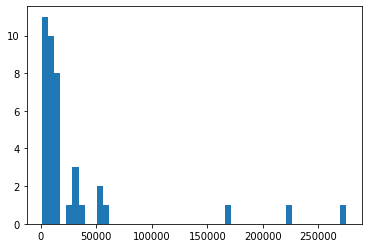
\includegraphics[keepaspectratio, scale=0.5]{img/g1.png}
      \subcaption{$G_1$}
      \label{g1}
    \end{minipage} &
    \begin{minipage}[t]{0.45\hsize}
      \centering
      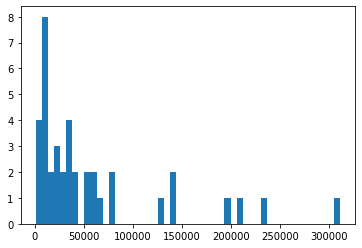
\includegraphics[keepaspectratio, scale=0.5]{img/g2.png}
      \subcaption{$G_2$}
      \label{g2}
    \end{minipage} \\

    \begin{minipage}[t]{0.45\hsize}
      \centering
      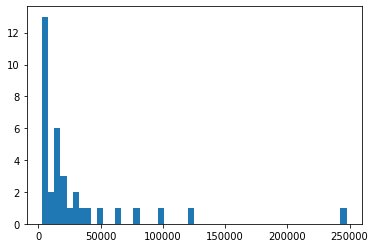
\includegraphics[keepaspectratio, scale=0.5]{img/g3.png}
      \subcaption{$G_3$}
      \label{g3}
    \end{minipage} &
    \begin{minipage}[t]{0.45\hsize}
      \centering
      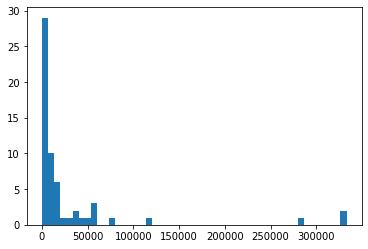
\includegraphics[keepaspectratio, scale=0.5]{img/g4.png}
      \subcaption{$G_4$}
      \label{g4}
    \end{minipage} \\
    \begin{minipage}[t]{0.45\hsize}
      \centering
      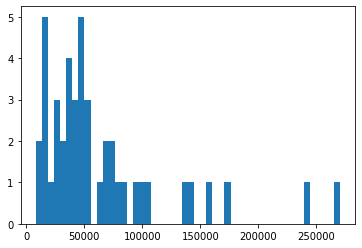
\includegraphics[keepaspectratio, scale=0.5]{img/g5.png}
      \subcaption{$G_5$}
      \label{g5}
    \end{minipage} &
    \begin{minipage}[t]{0.45\hsize}
      \centering
      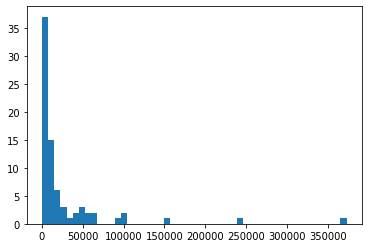
\includegraphics[keepaspectratio, scale=0.5]{img/g6.png}
      \subcaption{$G_6$}
      \label{g6}
    \end{minipage} \\

    \begin{minipage}[t]{0.45\hsize}
      \centering
      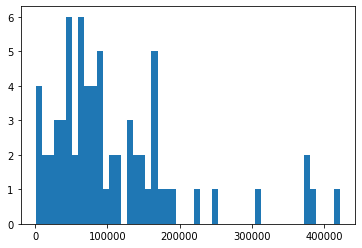
\includegraphics[keepaspectratio, scale=0.5]{img/g7.png}
      \subcaption{$G_7$}
      \label{g7}
    \end{minipage} &
    \begin{minipage}[t]{0.45\hsize}
      \centering
      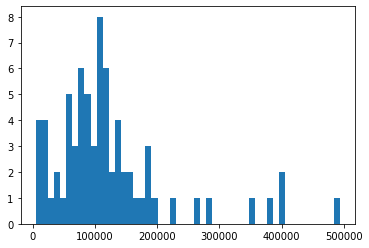
\includegraphics[keepaspectratio, scale=0.5]{img/g8.png}
      \subcaption{$G_8$}
      \label{g8}
    \end{minipage}
  \end{tabular}
  \caption{頂点の重み分布}
  \label{w_dist}
\end{figure}


\section{実験結果}

\subsection{人口制約を考慮しない列挙}

第3.3.1項にて述べた人口制約を考慮しない区割列挙アルゴリズムを,
各インスタンスにて行った結果を表\ref{out_normal}に示す.

\begin{table}[htbp]
  \caption{人口制約を考慮しない列挙}
  \label{out_normal}
  \centering
  \begin{tabular}{l||r|r|r|r}
    \hline
    Name & node & solve & time(sec) & memory(MB) \\
    \hline \hline
    $G_1$(Aomori) & 5{,}196 & 10{,}452{,}641 & 0.02 & 6 \\
    $G_2$(Miyagi) & 2{,}891 & 1.98E+10 & 0.01 & 4 \\
    $G_3$(Yamagata) & 2{,}672 & 490{,}516{,}246 & 0.01 & 4 \\
    $G_4$(Fukushima) & 233{,}446 & 1.51E+14 & 1{,}108.69 & 16{,}859 \\
    $G_5$(Ibaraki) & 10{,}757 & 3.24E+13 & 0.02 & 6 \\
    $G_6$(Nagano) & 48{,}612 & 3.82E+17 & 1.48 & 472 \\
    $G_7$(Aichi) & 1{,}145{,}106 & 3.02E+29 & 2.41 & 395 \\
    $G_8$(Osaka) & 955{,}147 & 1.73E+30 & 0.5 & 92 \\
    \hline
  \end{tabular}
\end{table}

表の各カラムについて,
Name はインスタンス名,
Node は構築したZDDのノード数,
solve はZDDにて列挙した解の個数,
time はZDD構築にかかった時間(単位は秒),
memory は計算機で使用したメモリ容量(単位は MB)
を表している.
人口制約がない場合,頂点に重みを保持する必要がないため,
$G_4$を除いて数秒以内に計算を終えることができた.
$G_4$はこの中で一番時間がかかるものの,計算時間や
メモリ使用量は一般的に許容範囲内である.
ただし,解の個数は非常に多く,分割数の最も多い
$G_8$では 1.73E+30 個という結果になった.

\subsection{許容格差定数$r$を用いた列挙}

許容格差定数$r=1.4$とし,各インスタンスごとに
重み下限$L$,重み上限$U$を第3.3.2項にて述べた計算方法
にて求めた.
それを用いてZDDを構築した結果を表\ref{out_r}に示す.

\begin{table}[htbp]
  \caption{$r=1.4$とした区割列挙}
  \label{out_r}
  \centering
  \begin{tabular}{l||r|r||r|r|r|r}
    \hline
    Name & $L$ & $U$ & node & solve & time(sec) & memory(MB) \\
    \hline \hline
    $G_1$(Aomori) & 325{,}785 & 509{,}759 & 23{,}749 & 668{,}154 & 2.25 & 405 \\
    $G_2$(Miyagi) & 348{,}787 & 596{,}814 & 6{,}581 & 40{,}106 & 3.38 & 652 \\
    $G_3$(Yamagata) & 281{,}059 & 439{,}776 & 319{,}171 & 7{,}493{,}473 & 33.81 & 6{,}702 \\
    $G_4$(Fukushima) & 353{,}649 & 585{,}129 & N/A & N/A & N/A & N/A \\
    $G_5$(Ibaraki) & 305{,}000 & 542{,}408 & 1{,}077{,}156 & 36{,}745{,}326 & 212.75 & 30{,}690 \\
    $G_6$(Nagano) & 310{,}304 & 530{,}966 & N/A & N/A & N/A & N/A \\
    $G_7$(Aichi) & 342{,}837 & 643{,}865 & N/A & N/A & N/A & N/A \\
    $G_8$(Osaka) & 337{,}316 & 637{,}772 & N/A & N/A & N/A & N/A \\
    \hline
  \end{tabular}
\end{table}

node,solve,time,memoryに値があるものは計算が出来ており,
N/A となっているものは,メモリ不足により計算が行えなかったことを
表している.
$G_1, G_2, G_3, G_5$では解を求められたが,
$G_4, G_6, G_7, G_8$では解を求められなかった.

\subsection{ヒューリスティクスを用いた列挙}

本節の実験では,第4章で述べたヒューリスティクスを用いて,各インスタンスにて
人口上下限制約$L, U$を求め,それを利用してZDDの構築を行なう.
ヒューリスティクスでの計算時間は,各120秒とし,10回実験を行った中で
最良の値を採用した.
各インスタンスの実験結果を表\ref{out_h}に示す.

\begin{table}[htbp]
  \caption{ヒューリスティクスを用いた区割列挙}
  \label{out_h}
  \centering
  \begin{tabular}{l||r|r||r|r|r|r}
    \hline
    Name & $L$ & $U$ & node & solve & time(sec) & memory(MB) \\
    \hline \hline
    $G_1$(Aomori) & 226{,}194 & 555{,}698 & 34{,}609 & 2{,}001{,}248 & 2.77 & 460 \\
    $G_2$(Miyagi) & 451{,}162 & 467{,}561 & 55 & 2 & 0.01 & 4 \\
    $G_3$(Yamagata) & 355{,}396 & 356{,}505 & 4{,}416 & 541 & 0.08 & 19 \\
    $G_4$(Fukushima) & 459{,}096 & 460{,}480 & N/A & N/A & N/A & N/A \\
    $G_5$(Ibaraki) & 391{,}937 & 419{,}212 & 1{,}340 & 390 & 0.02 & 6 \\
    $G_6$(Nagano) & 408{,}772 & 410{,}752 & 10{,}320 & 17{,}657 & 2.30 & 471 \\
    $G_7$(Aichi) & 359{,}399 & 553{,}700 & 1{,}847{,}085 & 1.29E+14 & 89.02 & 12{,}607 \\
    $G_8$(Osaka) & 424{,}530 & 569{,}011 & N/A & N/A & N/A & N/A \\
    \hline
  \end{tabular}
\end{table}

$G_1$を除いて,$L$と$U$の値の範囲を縮小することに成功した.
例えば,$G_6$において$r=1.4$を用いた場合は$U-L=220{,}662$
であるが,ヒューリスティクスを用いた場合$U-L=1{,}980$となり,
$1/100$程度の圧縮を行うことに成功した.
ZDDの構築においては,新たに$G_6, G_7$で解を求めることが出来た.
既存手法で解が求められているものについても,$G_1$以外は
4つの指標の値が大幅に削減されている.

\section{補足実験}

本節では,許容格差の値の変化によって解の個数
がどのように減るのかを確認するため,
第5.4.2項の実験から$G_3, G_5$において
$r$の値を細かく変化させ,
区割列挙を行った場合について検証を行った.
表\ref{table:g3_r}は$G_3$について,
表\ref{table:g5_r}は$G_5$についての
実験結果である.

\begin{table}[htbp]
  \caption{$G_3$で$r$を変化させた列挙}
  \label{table:g3_r}
  \centering
  \begin{tabular}{l||r|r|r|r}
    \hline
    $r$ & node & solve & time(sec) & memory(MB) \\
    \hline \hline
    1.40 & 319{,}171 & 7{,}493{,}473 &	33.89 &	6{,}702 \\
    1.35 & 289{,}106 &	5{,}873{,}171 &	27.25 &	5{,}164 \\
    1.30 & 255{,}214	& 4{,}403{,}896	& 22.02	& 3{,}972 \\
    1.25 & 222{,}857	& 3{,}111{,}414	& 15.99	& 2{,}791 \\
    1.20 & 188{,}371	& 2{,}014{,}623	& 10.92	& 1{,}896 \\
    1.15 & 152{,}860	& 1{,}146{,}740	& 6.96	& 1{,}133 \\
    1.10 & 111{,}220	& 527{,}439	& 3.64	& 570 \\
    1.05 & 67{,}194	& 135{,}951	& 1.36	& 212 \\
    1.025 & 40{,}548	& 36{,}118	& 0.61	& 106 \\
    1.010 & 19{,}378	& 6{,}503 & 0.27 & 54 \\
    \hline
  \end{tabular}
\end{table}

\begin{table}[htbp]
  \caption{$G_5$で$r$を変化させた列挙}
  \label{table:g5_r}
  \centering
  \begin{tabular}{l||r|r|r|r}
    \hline
    $r$ & node & solve & time(sec) & memory(MB) \\
    \hline \hline
    1.40	& 1{,}077{,}156	& 36{,}745{,}326 & 212.75	& 30{,}690 \\
    1.35	& 687{,}919	& 17{,}015{,}647 & 101.19	& 16{,}703 \\
    1.30	& 405{,}073	& 7{,}114{,}993	& 49.12 & 7{,}968 \\
    1.25	& 229{,}884	& 2{,}594{,}285	& 19.28 & 3{,}287 \\
    1.20	& 104{,}224	& 746{,}808	& 6.15	& 1{,}079 \\
    1.15	& 39{,}771	& 138{,}923	& 1.64	& 284 \\
    1.10	& 10{,}311	& 8{,}305	& 0.26	& 43 \\
    1.05	& 1{,}154	& 169	& 0.03	& 8 \\
    1.025	& 0	& 0	& 0.02	& 6 \\
    \hline
  \end{tabular}
\end{table}

どちらのインスタンスについても,解が存在する限り
$r$の値を小さくすればするほど,
4つの指標の値が削減されることがわかった.

\section{考察}

人口制約を考慮しない列挙は,実行時間やメモリ使用量のパフォーマンス
が行った実験の中で最もよく,全てのインスタンスにおいて解を得ることが出来た.
$G_4$の実行が遅い点については,インスタンスのグラフのサイズが大きいことに加え,
グラフの形状上,フロンティアのサイズが大きくなってしまったことが原因だと考えられる.
人口制約を考慮しない列挙は解の個数が非常に多く,ノードを参照しても各部分グラフの重みを保持していないため,
ZDDの終端から解の一票の格差を測ることが不可能である.
よって,選挙区割を見つける用途では実用的ではないことがわかった.

許容格差定数$r$を用いた列挙だが,$r=1.4$のときには,
ZDDのノード数が大幅に増加することからメモリ不足になり,
頂点数や辺数,選挙区数が大きいインスタンスでは解を得られなかった.
ただし,今回解を導出できた$G_5$より頂点の数が少ない都道府県は
47個中30個存在することから,$r=1.4$のままで
少なくとも過半数の都道府県は区割の列挙ができると考えられる.

ヒューリスティクスを用いた列挙では,$G_2, G_3,$ $ G_5, G_6$で
導出した$L$と$U$の値がほぼ一致しており,
この上下限制約を満たす選挙区割の個数も少ないことから,
最適解に近い区割を導出できたことがわかる.
$L$と$U$の値の差がないとき,ZDDの枝刈りがよく働くため
実行時間,メモリ使用量の双方で非常に良い結果が得られている.
しかし,$G_1$と$G_7$は$L$と$U$の差が大きく,
ZDDで列挙した解の個数も大きいことから,
ヒューリスティクス解は質の悪い局所解に陥っている可能性が高い.
また,例外として$G_4$は$U-L=1384$と非常に小さい値であるにも
関わらず,解を得ることが出来なかった.これも
グラフの形状からフロンティアのサイズが大きくなることが原因である.
さらに,$G_8$においては,最適解の選挙区の最大人口を最小人口で割った値が
およそ1.330ということが知られており,
ヒューリスティクスの結果が$U/L\fallingdotseq1.340$であることから
最適な選挙区割における$L$と$U$を導出したとしても,
ZDDを構築することはできないと考えられる.
このようなインスタンスでZDDで列挙をする場合は,
$U$と$L$の値を変化させる以外の手法を考える必要がある.
